\documentclass[a4paper]{article}
\usepackage[a4paper,top=2cm,bottom=2cm,left=1cm,right=1cm,marginparwidth=1.75cm]{geometry}
% \usepackage[spanish]{babel}
% \selectlanguage{spanish}
% \usepackage[utf8]{inputenc}
% \usepackage[T1]{fontenc}
% \usepackage[spanish]{babel}

% \usepackage[T1]{fontenc}
\usepackage{graphicx} %Paquete para usar imagenes
\usepackage{listings}
\usepackage{xcolor}
\usepackage{tcolorbox}

\definecolor{background}{HTML}{E7EBF4}
\definecolor{bg}{HTML}{1a1b26}
\definecolor{fg}{HTML}{a9b1d6}
\definecolor{comment}{HTML}{848cb5}
\definecolor{cyan}{HTML}{82aaff}
\definecolor{orange}{HTML}{ff9e64}
\definecolor{yellow}{HTML}{e9d78e}
\definecolor{purple}{HTML}{c792ea}
\definecolor{green}{HTML}{7fdbca}
\definecolor{numbers}{HTML}{9854f1}
\definecolor{keyword}{HTML}{9854f1}

\lstset{
    showspaces=false, % Evita mostrar espacios en blanco como ␣
    showstringspaces=false,
    inputencoding=utf8,
    extendedchars=true,
    literate=%
    {á}{{\'a}}1
    {é}{{\'e}}1
    {í}{{\'i}}1
    {ó}{{\'o}}1
    {ú}{{\'u}}1
    {ñ}{{\~n}}1
}
\lstdefinestyle{mystyle}{
    language=Python,
    basicstyle=\ttfamily,
    keywordstyle=\color{keyword},
    commentstyle=\color{comment},
    numbers=none,
    numberstyle=\tiny\color{numbers},
    frame=none,
    breaklines=true,
    % showstringspaces=false
    xleftmargin=0mm,
    xrightmargin=0mm,
}

\lstset{style=mystyle}

\newtcolorbox{mycodebox}[1][]{
    arc=7pt,  % Radio de las esquinas redondeadas
    colback=background,  % Color de fondo del cuadro
    boxrule=0.5pt,  % Grosor de la línea del cuadro
    colframe=background,
    width=0.8\textwidth,   % Anchura del cuadro
    % height=5cm,            % Altura del cuadro
    % breakable,
    #1  % Otras opciones personalizadas que puedas necesitar
}


\newtcolorbox{mycodeboxl}[1][]{
    arc=7pt,  % Radio de las esquinas redondeadas
    colback=background,  % Color de fondo del cuadro
    boxrule=0.5pt,  % Grosor de la línea del cuadro
    colframe=background,
    width=0.94\textwidth,   % Anchura del cuadro
    % height=5cm,            % Altura del cuadro
    % breakable,
    #1  % Otras opciones personalizadas que puedas necesitar
}

% Documento
\begin{document}
\newgeometry{left=3cm,right=3cm,top=2cm,bottom=2cm}
\begin{titlepage}

%--------------- Nuevo comendo de linea ----------------->
\newcommand{\linea}{\rule{\linewidth}{0.7mm}} 
\center
%--------------- Universidad, facultad y carrera ----------------->
\textbf{\Large UNIVERSIDAD NACIONAL DE SAN ANTONIO ABAD DEL CUSCO}\\[0.2cm]
\textbf{\Large FACULTAD DE INGENIERÍA ELÉCTRICA, ELECTRÓNICA,INFORMÁTICA Y MECÁNICA}\\[0.2cm]
\textbf{\Large INGENIERÍA INFORMÁTICA Y DE SISTEMAS\\[0.6cm]}

%--------------- Escudos png ----------------->

\includegraphics[width=8cm]{src/escudo-unsaac.png}
\vfill

%--------------- Tema ----------------->
\linea
\\[0.3cm]
% \vfill
\textbf{\LARGE Guía de Laboratorio 1 - Algoritmos para trazo de lineas}\\[0.2cm]
\linea \\
\vfill

%--------------- Integrantes ----------------->
\textit{\Large Alumno:}\\
%Integrantes del grupo
    \textbf{\large Ian Logan Will Quispe Ventura}\\
    \textit{211359}\\
    % \vfill

%--------------- Profesor y curso ----------------->
\vspace{0.3cm}
    \textit{\Large Docente:}\\
    \textbf{\large Hector Eduardo Ugarte Rojas}\\
\vspace{0.5cm}
    \textit{\Large Curso:}\\
    \textbf{\large Computación Gráfica}\\
    \vfill

\vspace{0.4cm}
    \textbf{\Large Cusco - Perú }\\
    \textbf{\large 2023 - II }\\
    \newpage
    \end{titlepage}

\restoregeometry
\newpage
% •·•·•·•·•·•••·•·•·•·•·•·•·•·•·•·•·•·•·•·•·•·•·•·•·•·•.,..,
% \section{Funcionamiento del algoritmo DDA}
\Large{\textbf{Funcionamiento del algoritmo DDA}}\\[0.5cm]
El código original impedía que ciertas lineas se dibujaran, estas lineas tenían a la pendiente mayor que 1 o menor que -1. Para solucionarlo usarmos esta versión mejorada.
\begin{center}
\begin{mycodebox}
\begin{lstlisting}
def DDA(x0, y0, x1, y1):
    dx = x1 - x0
    dy = y1 - y0

    if abs(dx) >= abs(dy):
        steps = abs(dx)
    else:
        steps = abs(dy)

    x_increment = dx / steps
    y_increment = dy / steps

    x = x0
    y = y0

    for _ in range(steps + 1):
        plot(int(x), int(y))
        x += x_increment
        y += y_increment
\end{lstlisting}
\end{mycodebox}
\end{center}
Modulo Display para DDA
\begin{center}
\begin{mycodebox}
\begin{lstlisting}
def display_DDA():
    glClear(GL_COLOR_BUFFER_BIT)
    glColor3f(1.0, 0.0, 0.0)
    DDA(100, 100, 450, 450)
    DDA(200, 450, 450, 450)
    glFlush()
\end{lstlisting}
\end{mycodebox}
\end{center}
\newpage
Gráfico generado\\

\includegraphics[width=15cm]{src/bresenham.png}
\newpage
% \newpage

\Large{\textbf{Funcionamiento del algoritmo Bresenham}}\\[0.5cm]
Modulo Display para Bresenham
\begin{center}
\begin{mycodebox}
\begin{lstlisting}
def display_Bresenham():
    glClear(GL_COLOR_BUFFER_BIT)
    glColor3f(1.0, 0.0, 0.0)
    Bresenham(100, 100, 450, 450)
    Bresenham(200, 450, 450, 450)
    glFlush()
\end{lstlisting}
\end{mycodebox}
\end{center}
Gráfico generado\\

\includegraphics[width=15cm]{src/bresenham.png}
\newpage

\Large{\textbf{Funcionamiento del algoritmo Punto Medio}}\\[0.5cm]
Modulo Display para Punto Medio 
\begin{center}
\begin{mycodebox}
\begin{lstlisting}
def display_PtoMedio():
    glClear(GL_COLOR_BUFFER_BIT)
    glColor3f(1.0, 0.0, 0.0)
    PtoMedio(100, 100, 450, 450)
    PtoMedio(200, 450, 450, 450)
    glFlush()
\end{lstlisting}
\end{mycodebox}
\end{center}
Gráfico generado\\

\includegraphics[width=15cm]{src/PtoMedio.png}\\
\newpage

\Large{\textbf{Algoritmo para dibujar 5 lineas y mostrar la intersección}}\\[0.5cm]

% \section{}

Primero  creamos una lista y guardamos en ella los puntos de las lineas.
\begin{center}
\begin{mycodebox}
\begin{lstlisting}
# Declarar lista de todos los puntos que conforman las lineas
lista_puntos = []

def DDA(x0, y0, x1, y1):
    m = (y1 - y0) / (x1 - x0)
    y = y0
    for x in range(x0, x1 + 1):
        plot(x, int(y))
        # Anadir los puntos a la lista
        lista_puntos.append((x, int(y)))
        y = y + m
\end{lstlisting}
\end{mycodebox}
\end{center}
% \newpage
En la función display dibujaremos las 5 lineas requeridas, con valores aleatorios en los puntos.
\begin{center}
\begin{mycodebox}
\begin{lstlisting}
def display():
    glClear(GL_COLOR_BUFFER_BIT)
    glColor3f(1.0, 0.0, 0.0)

    # Limpiar la lista de puntos
    lista_puntos.clear()

    # Dibujar 5 líneas aleatorias
    for _ in range(5):
        x0 = random.randint(10, 150)
        y0 = random.randint(10, 150)
        x1 = random.randint(250, 499)
        y1 = random.randint(250, 499)
        DDA(x0, y0, x1, y1)
\end{lstlisting}
\end{mycodebox}
\end{center}
    % \includegraphics[width=15cm]{src/pelicula.png}\\
% \newpage

Los puntos se guardan en una lista, en esta verificaremos los puntos repetidos que serán las intersecciones.\\ 
Dibujaremos puntos de otro color con esas coordenadas para resaltar las intersecciones.
\begin{center}
    
\begin{mycodeboxl}
\begin{lstlisting}
    # Lista para los puntos duplicado
    interseccion = []

    # Crear un conjunto para llevar un registro de los puntos únicos que hemos visto
    puntos_unicos = set()

    # Recorremos la lista de puntos
    for punto in lista_puntos:
        if punto in puntos_unicos:
            # Si los puntos se encuentran en el conjunto, se añaden a la lista intersección. Inicialmente no hay elementos en el conjunto 
            interseccion.append(punto)
        else:
            # Si no se encuentra el punto en el conjunto, entonces este se añade al mismo conjunto que se utilicará en la próxima iteración
            puntos_unicos.add(punto)
    print("Puntos de intersección de las lineas:", interseccion)

    # Pintar de negro los puntos de intersección
    glColor3f(0.0, 0.0, 0.0)
    glPointSize(3)

    # Recorrer la lista de duplicados para dibujarlos 
    for punto in interseccion:
        x, y = punto
        plot(x, y)
    glPointSize(1)
    glFlush()
\end{lstlisting}
\end{mycodeboxl}
\end{center}

\newpage
\Large{\textbf{Capturas de la ventana de gráficos}}\\[0.5cm]
\begin{center}
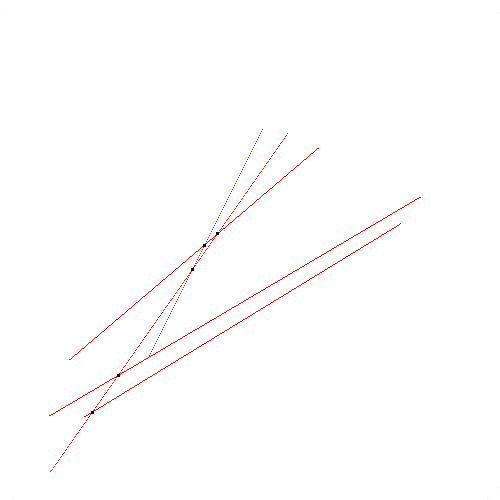
\includegraphics[width=8cm]{src/1.png}
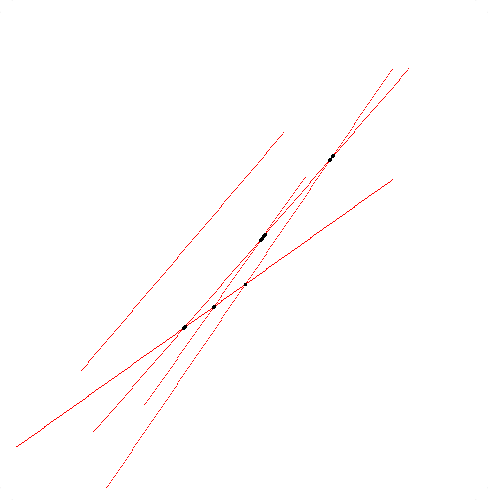
\includegraphics[width=8cm]{src/2.png}\\

\includegraphics[width=8cm]{src/3.png}

\includegraphics[width=8cm]{src/4.png}
\end{center}
\end{document}
